\documentclass[11pt]{article}\usepackage[]{graphicx}\usepackage[]{color}
%% maxwidth is the original width if it is less than linewidth
%% otherwise use linewidth (to make sure the graphics do not exceed the margin)
\makeatletter
\def\maxwidth{ %
  \ifdim\Gin@nat@width>\linewidth
    \linewidth
  \else
    \Gin@nat@width
  \fi
}
\makeatother

\definecolor{fgcolor}{rgb}{0.345, 0.345, 0.345}
\newcommand{\hlnum}[1]{\textcolor[rgb]{0.686,0.059,0.569}{#1}}%
\newcommand{\hlstr}[1]{\textcolor[rgb]{0.192,0.494,0.8}{#1}}%
\newcommand{\hlcom}[1]{\textcolor[rgb]{0.678,0.584,0.686}{\textit{#1}}}%
\newcommand{\hlopt}[1]{\textcolor[rgb]{0,0,0}{#1}}%
\newcommand{\hlstd}[1]{\textcolor[rgb]{0.345,0.345,0.345}{#1}}%
\newcommand{\hlkwa}[1]{\textcolor[rgb]{0.161,0.373,0.58}{\textbf{#1}}}%
\newcommand{\hlkwb}[1]{\textcolor[rgb]{0.69,0.353,0.396}{#1}}%
\newcommand{\hlkwc}[1]{\textcolor[rgb]{0.333,0.667,0.333}{#1}}%
\newcommand{\hlkwd}[1]{\textcolor[rgb]{0.737,0.353,0.396}{\textbf{#1}}}%

\usepackage{framed}
\makeatletter
\newenvironment{kframe}{%
 \def\at@end@of@kframe{}%
 \ifinner\ifhmode%
  \def\at@end@of@kframe{\end{minipage}}%
  \begin{minipage}{\columnwidth}%
 \fi\fi%
 \def\FrameCommand##1{\hskip\@totalleftmargin \hskip-\fboxsep
 \colorbox{shadecolor}{##1}\hskip-\fboxsep
     % There is no \\@totalrightmargin, so:
     \hskip-\linewidth \hskip-\@totalleftmargin \hskip\columnwidth}%
 \MakeFramed {\advance\hsize-\width
   \@totalleftmargin\z@ \linewidth\hsize
   \@setminipage}}%
 {\par\unskip\endMakeFramed%
 \at@end@of@kframe}
\makeatother

\definecolor{shadecolor}{rgb}{.97, .97, .97}
\definecolor{messagecolor}{rgb}{0, 0, 0}
\definecolor{warningcolor}{rgb}{1, 0, 1}
\definecolor{errorcolor}{rgb}{1, 0, 0}
\newenvironment{knitrout}{}{} % an empty environment to be redefined in TeX

\usepackage{alltt}
\usepackage{amsmath}
\usepackage{stmaryrd}
\usepackage{bbm}
\usepackage{amsmath}
\usepackage{mathtools}
\usepackage{pdfpages}
\usepackage{breqn}

\newcount\colveccount
\newcommand*\colvec[1]{
        \global\colveccount#1
        \begin{pmatrix}
        \colvecnext
}
\def\colvecnext#1{
        #1
        \global\advance\colveccount-1
        \ifnum\colveccount>0
                \\
                \expandafter\colvecnext
        \else
                \end{pmatrix}
        \fi
}
\newcommand{\argmin}{\arg\!\min}

\author{Thibault Doutre, Student ID 26980469}
\title{STAT230 HW 3 \\
University of California, Berkeley}
\date{\today}
\IfFileExists{upquote.sty}{\usepackage{upquote}}{}
\begin{document}
\maketitle

\section{} 
Here is the code to generate the data, using the bivariate normal relationship $Y=\rho X +\sqrt{1-\rho^2} Z$, for $Z$ being standard normal.
\begin{knitrout}
\definecolor{shadecolor}{rgb}{0.969, 0.969, 0.969}\color{fgcolor}\begin{kframe}
\begin{alltt}
\hlstd{generate_data} \hlkwb{=} \hlkwa{function}\hlstd{(}\hlkwc{n} \hlstd{=} \hlnum{100}\hlstd{)\{}
  \hlcom{# Define parameters}
  \hlstd{rho} \hlkwb{=} \hlnum{0.7}
  \hlstd{mu1}\hlkwb{=}\hlnum{180}\hlstd{; s1}\hlkwb{=}\hlnum{40}\hlstd{; mu2}\hlkwb{=}\hlnum{66}\hlstd{; s2}\hlkwb{=}\hlnum{3}

  \hlcom{# Define X, Y and Z with the bivariate normal relationship}
  \hlstd{X} \hlkwb{=} \hlkwd{rnorm}\hlstd{(n)}
  \hlstd{Z} \hlkwb{=} \hlkwd{rnorm}\hlstd{(n)}
  \hlstd{eps} \hlkwb{=} \hlkwd{sqrt}\hlstd{(}\hlnum{1}\hlopt{-}\hlstd{rho}\hlopt{^}\hlnum{2}\hlstd{)} \hlopt{*} \hlstd{Z}
  \hlstd{Y} \hlkwb{=} \hlstd{rho} \hlopt{*} \hlstd{X} \hlopt{+} \hlstd{eps}

  \hlcom{# Adjust means and variances}
  \hlstd{Y} \hlkwb{=} \hlstd{(Y}\hlopt{-}\hlkwd{mean}\hlstd{(Y))}\hlopt{/}\hlkwd{sd}\hlstd{(Y)}\hlopt{*}\hlstd{s2}\hlopt{+}\hlstd{mu2}
  \hlstd{X} \hlkwb{=} \hlstd{(X}\hlopt{-}\hlkwd{mean}\hlstd{(X))}\hlopt{/}\hlkwd{sd}\hlstd{(X)}\hlopt{*}\hlstd{s1}\hlopt{+}\hlstd{mu1}

  \hlcom{# Adjust rho by transforming Y}
  \hlstd{rho_hat} \hlkwb{=} \hlkwd{cor}\hlstd{(X,Y)}
  \hlstd{a} \hlkwb{=} \hlstd{s1}\hlopt{^}\hlnum{4}\hlopt{*}\hlstd{(rho}\hlopt{^}\hlnum{2}\hlopt{-}\hlnum{1}\hlstd{)}
  \hlstd{b} \hlkwb{=} \hlnum{2}\hlopt{*}\hlstd{rho_hat}\hlopt{*}\hlstd{s1}\hlopt{^}\hlnum{3}\hlopt{*}\hlstd{s2}\hlopt{*}\hlstd{(rho}\hlopt{^}\hlnum{2}\hlopt{-}\hlnum{1}\hlstd{)}
  \hlstd{c} \hlkwb{=} \hlstd{(rho}\hlopt{^}\hlnum{2}\hlopt{-}\hlstd{rho_hat}\hlopt{^}\hlnum{2}\hlstd{)}\hlopt{*}\hlstd{s2}\hlopt{^}\hlnum{2}\hlopt{*}\hlstd{s1}\hlopt{^}\hlnum{2}
  \hlstd{delta} \hlkwb{=} \hlstd{b}\hlopt{^}\hlnum{2}\hlopt{-}\hlnum{4}\hlopt{*}\hlstd{a}\hlopt{*}\hlstd{c}
  \hlstd{correction} \hlkwb{=} \hlstd{(}\hlopt{-}\hlstd{b}\hlopt{-}\hlkwd{sqrt}\hlstd{(delta))}\hlopt{/}\hlstd{(}\hlnum{2}\hlopt{*}\hlstd{a)}
  \hlstd{Y}\hlkwb{=}\hlstd{Y}\hlopt{+}\hlstd{correction}\hlopt{*}\hlstd{X}

  \hlcom{# Adjust means and variances}
  \hlstd{Y} \hlkwb{=} \hlstd{(Y}\hlopt{-}\hlkwd{mean}\hlstd{(Y))}\hlopt{/}\hlkwd{sd}\hlstd{(Y)}\hlopt{*}\hlstd{s2}\hlopt{+}\hlstd{mu2}
  \hlstd{X} \hlkwb{=} \hlstd{(X}\hlopt{-}\hlkwd{mean}\hlstd{(X))}\hlopt{/}\hlkwd{sd}\hlstd{(X)}\hlopt{*}\hlstd{s1}\hlopt{+}\hlstd{mu1}

  \hlcom{# Put into data frame}
  \hlstd{df} \hlkwb{=} \hlkwd{data.frame}\hlstd{(}\hlkwc{WT} \hlstd{= Y,}
                  \hlkwc{HT} \hlstd{= X,}
                  \hlkwc{BMI} \hlstd{=} \hlnum{703} \hlopt{*} \hlstd{Y} \hlopt{/} \hlstd{X}\hlopt{^}\hlnum{2}\hlstd{)}

  \hlcom{# Output}
  \hlkwd{return}\hlstd{(}\hlkwd{list}\hlstd{(}\hlkwc{df}\hlstd{=df,}\hlkwc{rho}\hlstd{=rho,}\hlkwc{eps}\hlstd{=eps))}
\hlstd{\}}
\hlstd{data} \hlkwb{=} \hlkwd{generate_data}\hlstd{()}

\hlstd{df} \hlkwb{=} \hlstd{data}\hlopt{$}\hlstd{df}
\hlstd{M}\hlkwb{=}\hlstd{df[,}\hlnum{1}\hlopt{:}\hlnum{2}\hlstd{]}
\hlstd{rho} \hlkwb{=} \hlstd{data}\hlopt{$}\hlstd{rho}
\hlstd{eps} \hlkwb{=} \hlstd{data}\hlopt{$}\hlstd{eps}
\end{alltt}
\end{kframe}
\end{knitrout}
In order to adjust the correlation of the random variables $X$ and $Y$, I defined:
\begin{align}
\hat{\rho} &= \frac{cov(X,Y)}{\sigma_X \sigma_Y} \\
\end{align}
And a cosntant $correction$ such that:
\begin{align}
\rho &= \frac{cov(X,Y+correction*X)}{\sigma_X \sigma_Y}
\end{align}
I find the correction coefficient by finding the negative solution of the second order equation:
\begin{align}
\rho &= \frac{cov(X,Y+correction*X)}{\sigma_X \sigma_Y} \\
\rho &= \frac{cov(X,Y)+correction*\sigma_X^2}{\sigma_X \sqrt{correction^2 \sigma_X^2 + 2 correction *cov(X,Y)+ \sigma_Y^2}}
\end{align}

Which is equivalent to:
\begin{dmath}
(\rho^2-1)\sigma_X^4 *correction^2+ 2\hat{\rho}\sigma_X^3*\sigma_Y^3*(\rho^2-1)*correction\\
+(\rho^2-\hat{\rho}^2)*\sigma_Y^2*\sigma_X^2 = 0
\end{dmath}
Then, we can easily solve this equation and find the corresponding $correction$ to adjust the $\hat{\rho}$ to be $\rho$.

We can see the result by displaying the correlation matrix.

\begin{knitrout}
\definecolor{shadecolor}{rgb}{0.969, 0.969, 0.969}\color{fgcolor}\begin{kframe}
\begin{alltt}
\hlcom{# Correlation and covariance matrices}
\hlkwd{cor}\hlstd{(M)}
\end{alltt}
\begin{verbatim}
##     WT  HT
## WT 1.0 0.7
## HT 0.7 1.0
\end{verbatim}
\begin{alltt}
\hlkwd{cov}\hlstd{(M)}
\end{alltt}
\begin{verbatim}
##    WT   HT
## WT  9   84
## HT 84 1600
\end{verbatim}
\begin{alltt}
\hlcom{# Mean of variables}
\hlkwd{mean}\hlstd{(df}\hlopt{$}\hlstd{WT)}
\end{alltt}
\begin{verbatim}
## [1] 66
\end{verbatim}
\begin{alltt}
\hlkwd{mean}\hlstd{(df}\hlopt{$}\hlstd{HT)}
\end{alltt}
\begin{verbatim}
## [1] 180
\end{verbatim}
\end{kframe}
\end{knitrout}


\section{} 
\begin{knitrout}
\definecolor{shadecolor}{rgb}{0.969, 0.969, 0.969}\color{fgcolor}\begin{kframe}
\begin{alltt}
\hlstd{lm.fit} \hlkwb{=} \hlkwd{lm}\hlstd{(WT} \hlopt{~} \hlstd{.,} \hlkwc{data} \hlstd{= df)}
\hlstd{beta} \hlkwb{=} \hlstd{lm.fit}\hlopt{$}\hlstd{coefficients}
\end{alltt}
\end{kframe}
\end{knitrout}

False assumptions:

First X and Y are random variables, not observed values. Here we know $\beta$ and do observe $\epsilon$. 
The model is not linear itself, i.e. BMI is not a linear function of the columns of X.
The resuiduals are not gaussian. We can see it by plotting the object $lm.fit$.
\begin{knitrout}
\definecolor{shadecolor}{rgb}{0.969, 0.969, 0.969}\color{fgcolor}\begin{kframe}
\begin{alltt}
\hlkwd{par}\hlstd{(}\hlkwc{mfrow}\hlstd{=}\hlkwd{c}\hlstd{(}\hlnum{2}\hlstd{,}\hlnum{2}\hlstd{))}
\hlkwd{plot}\hlstd{(lm.fit)}
\end{alltt}
\end{kframe}
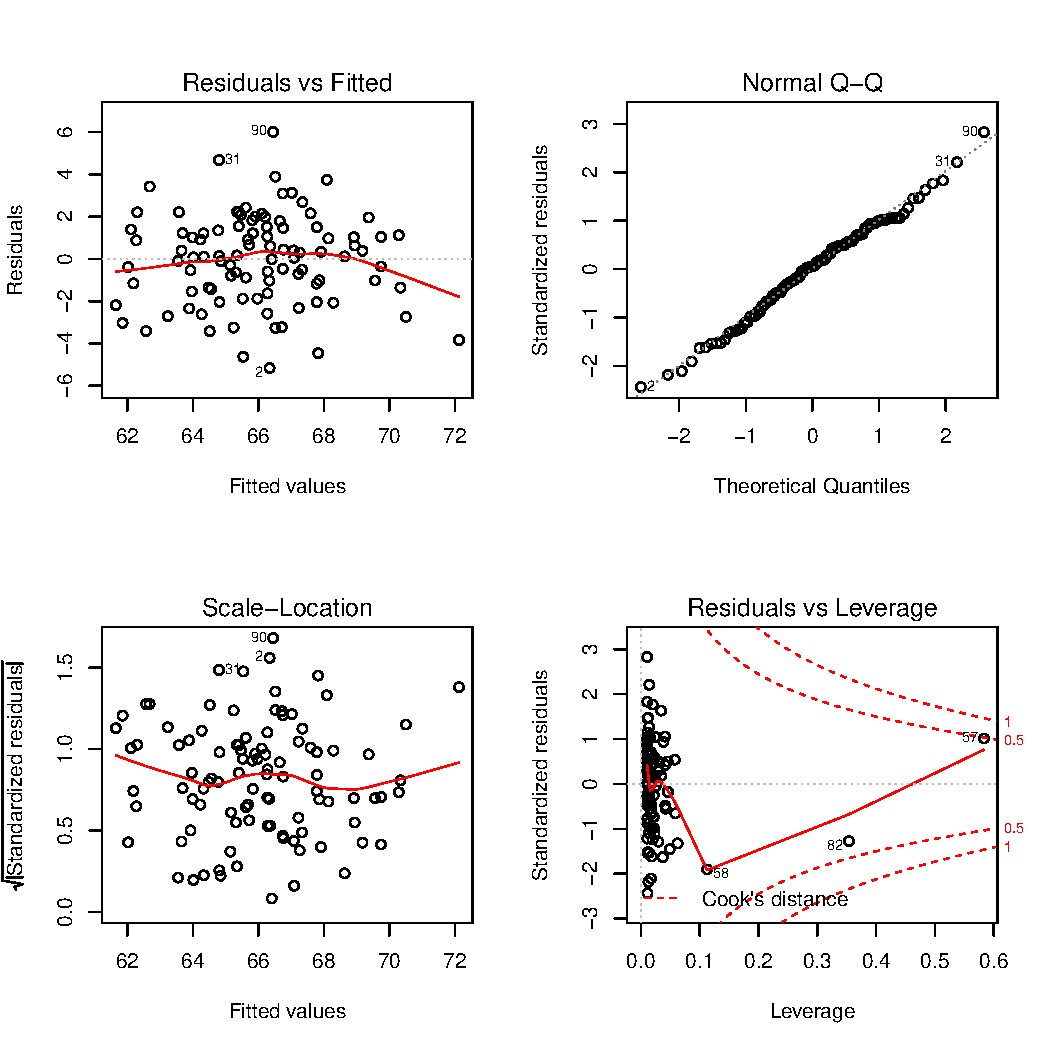
\includegraphics[width=\maxwidth]{figure/unnamed-chunk-4-1} 
\begin{kframe}\begin{alltt}
\hlkwd{par}\hlstd{(}\hlkwc{mfrow}\hlstd{=}\hlkwd{c}\hlstd{(}\hlnum{1}\hlstd{,}\hlnum{1}\hlstd{))}
\end{alltt}
\end{kframe}
\end{knitrout}

In particular, the sd of the residuals is not equal to 1:
\begin{knitrout}
\definecolor{shadecolor}{rgb}{0.969, 0.969, 0.969}\color{fgcolor}\begin{kframe}
\begin{alltt}
\hlkwd{sd}\hlstd{(lm.fit}\hlopt{$}\hlstd{residuals)}
\end{alltt}
\begin{verbatim}
## [1] 2.11417
\end{verbatim}
\end{kframe}
\end{knitrout}

\section{} 
The true value of $\beta_1$, the coefficient associated with the height $HT$, is $\rho*\frac{sd(WT)}{sd(HT)}$.
\begin{knitrout}
\definecolor{shadecolor}{rgb}{0.969, 0.969, 0.969}\color{fgcolor}\begin{kframe}
\begin{alltt}
\hlcom{# True value of beta}
\hlstd{beta_true} \hlkwb{=} \hlstd{rho}\hlopt{*}\hlkwd{sd}\hlstd{(df}\hlopt{$}\hlstd{WT)}\hlopt{/}\hlkwd{sd}\hlstd{(df}\hlopt{$}\hlstd{HT)}
\hlstd{beta_true}
\end{alltt}
\begin{verbatim}
## [1] 0.0525
\end{verbatim}
\begin{alltt}
\hlcom{# The simulated value of $\textbackslash{}beta_1$ is}
\hlstd{beta1} \hlkwb{=} \hlstd{beta[}\hlstr{"HT"}\hlstd{]}
\hlstd{beta1}
\end{alltt}
\begin{verbatim}
##         HT 
## 0.06237115
\end{verbatim}
\end{kframe}
\end{knitrout}

\section{} 

According to Theorem 2, page 43 of Freedman, OLS is conditionally unbiased, that is, $E(\hat{\beta}|X) = \beta$. Therefore, we should have $E(E(\hat{\beta}|X))=\beta$ i.e. $E(\hat{\beta})=\beta$. However here some assumptions for the OLS are not true. Therefore, the estimator could be biased.



\section{} 
\begin{knitrout}
\definecolor{shadecolor}{rgb}{0.969, 0.969, 0.969}\color{fgcolor}\begin{kframe}
\begin{alltt}
\hlstd{WT_hat} \hlkwb{=} \hlkwd{predict}\hlstd{(lm.fit)}
\hlstd{e} \hlkwb{=} \hlstd{df}\hlopt{$}\hlstd{WT}\hlopt{-}\hlstd{WT_hat}
\end{alltt}
\end{kframe}
\end{knitrout}
To see if the variables are correlated, wee look for some pattern in the plot of one against the other.
\begin{knitrout}
\definecolor{shadecolor}{rgb}{0.969, 0.969, 0.969}\color{fgcolor}\begin{kframe}
\begin{alltt}
\hlkwd{plot}\hlstd{(eps,df}\hlopt{$}\hlstd{HT)} \hlcom{# not correlated, seem to be independent}
\end{alltt}
\end{kframe}
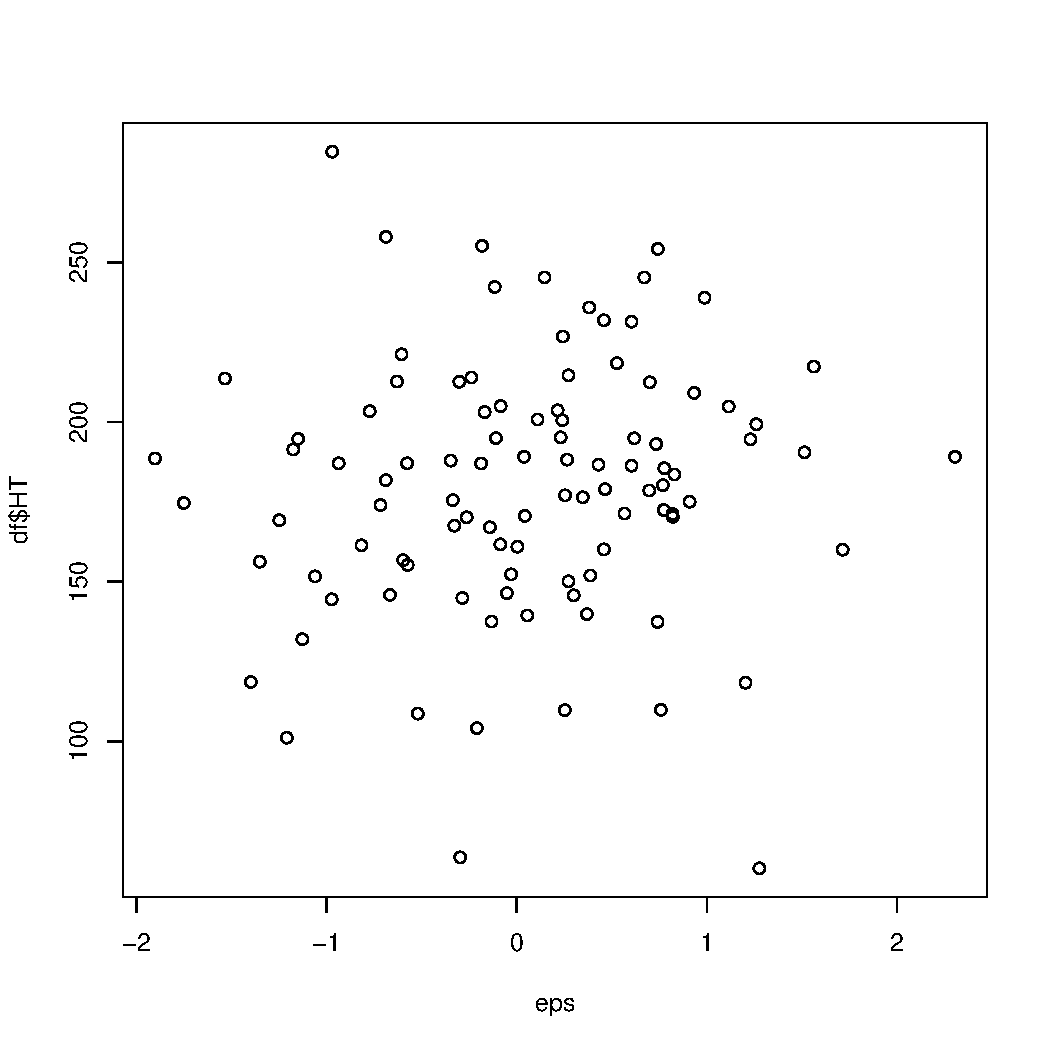
\includegraphics[width=\maxwidth]{figure/unnamed-chunk-8-1} 
\begin{kframe}\begin{alltt}
\hlkwd{plot}\hlstd{(eps,df}\hlopt{$}\hlstd{WT)} \hlcom{# positively correlated -> dependent}
\end{alltt}
\end{kframe}
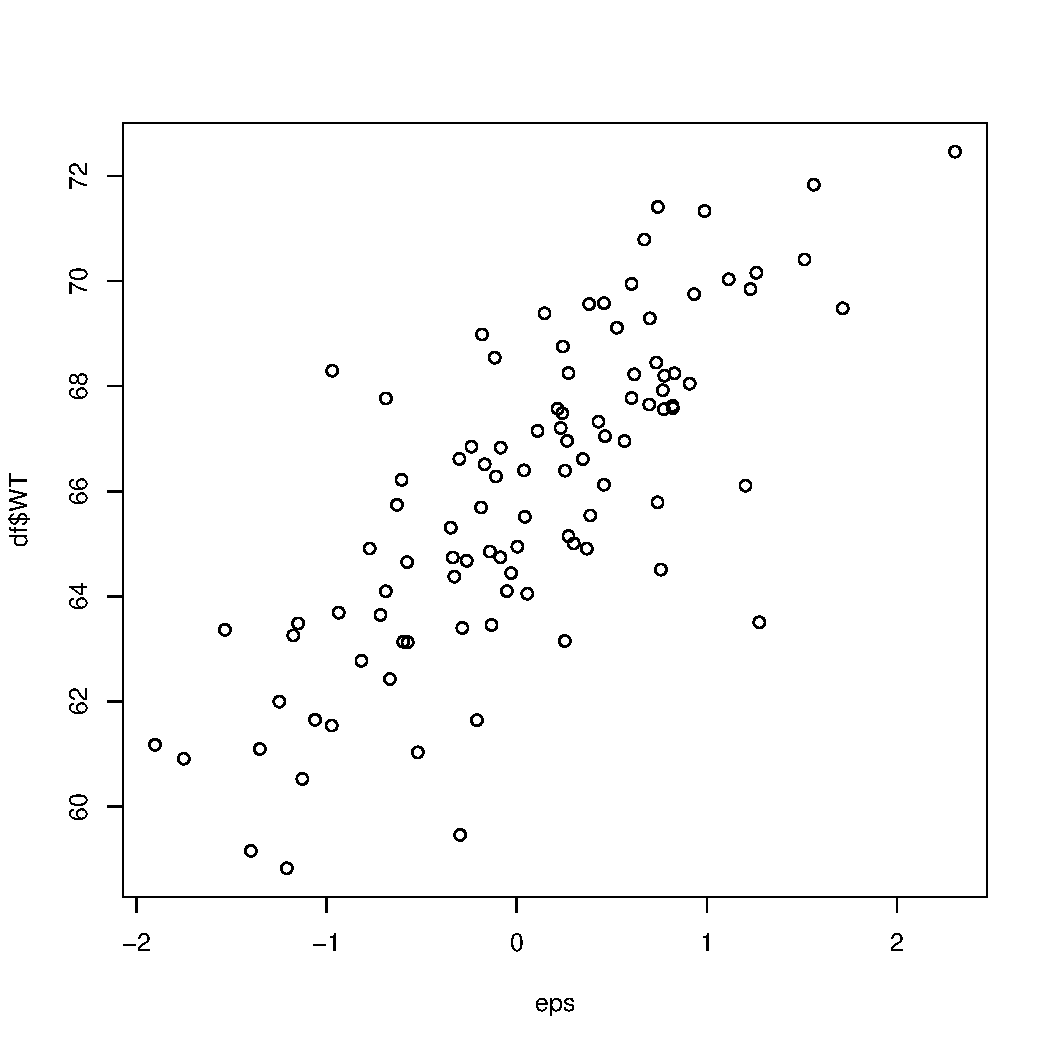
\includegraphics[width=\maxwidth]{figure/unnamed-chunk-8-2} 
\begin{kframe}\begin{alltt}
\hlkwd{plot}\hlstd{(e,df}\hlopt{$}\hlstd{WT)} \hlcom{# positively correlated -> dependent}
\end{alltt}
\end{kframe}
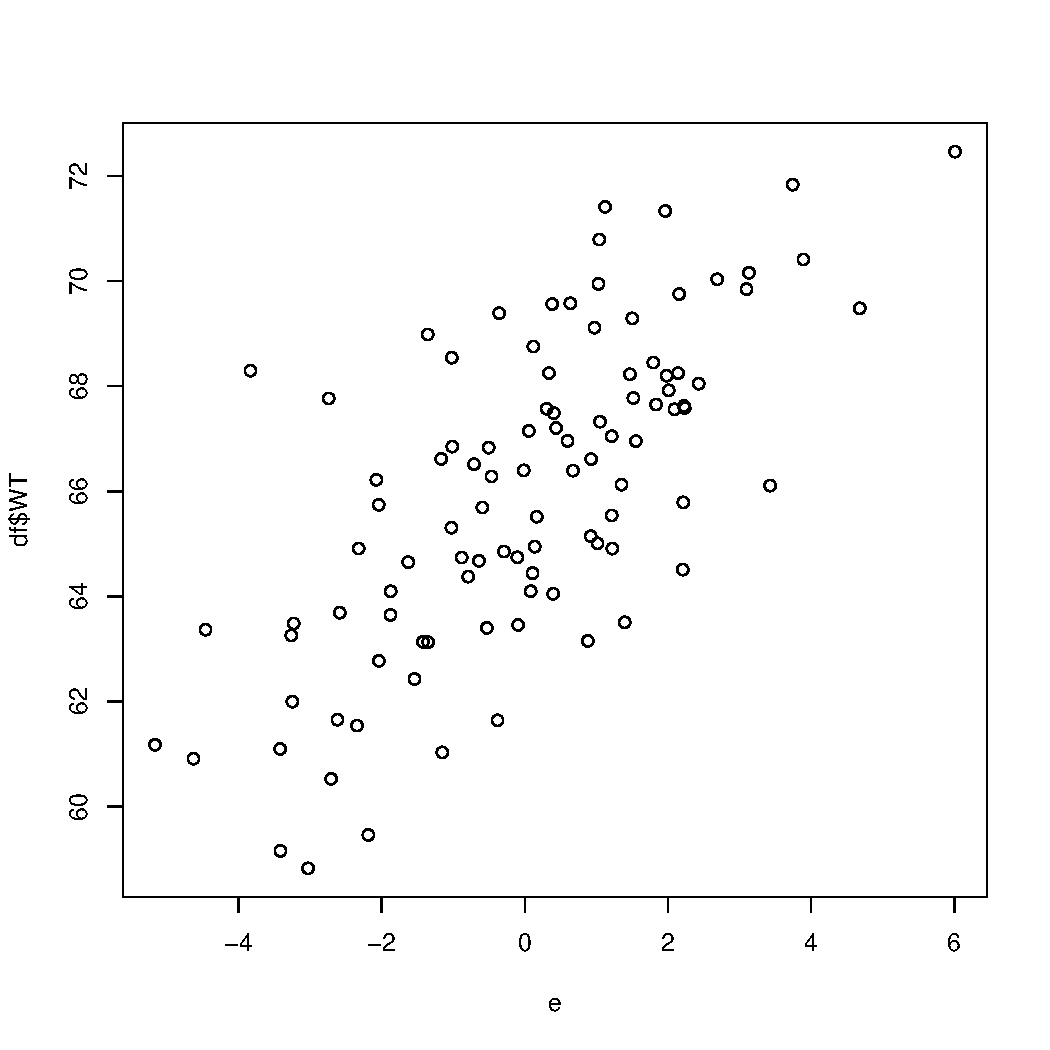
\includegraphics[width=\maxwidth]{figure/unnamed-chunk-8-3} 
\begin{kframe}\begin{alltt}
\hlkwd{plot}\hlstd{(e,df}\hlopt{$}\hlstd{HT)} \hlcom{# not correlated, seem to be independent}
\end{alltt}
\end{kframe}
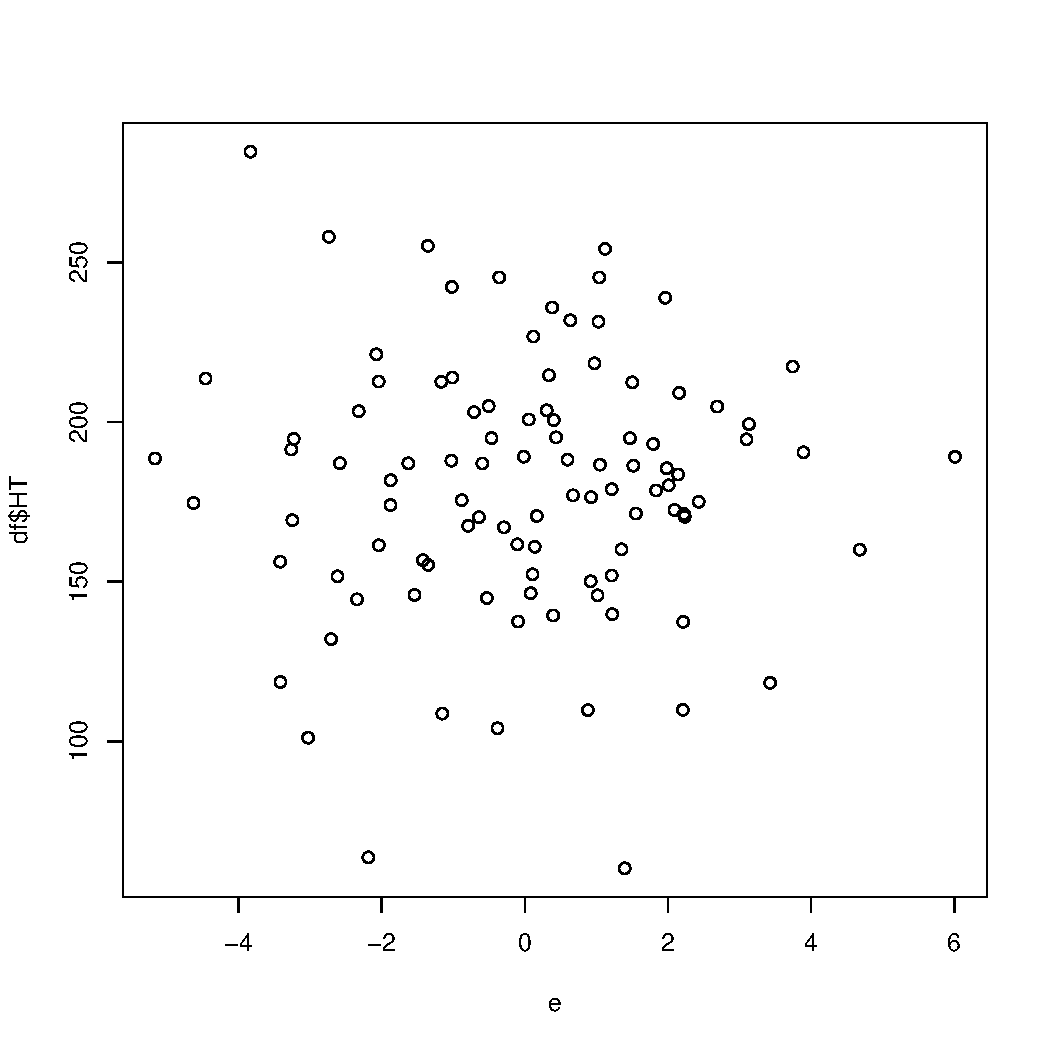
\includegraphics[width=\maxwidth]{figure/unnamed-chunk-8-4} 

\end{knitrout}
To see if two vectors are orthogonal, I compute their scalar product.
\begin{knitrout}
\definecolor{shadecolor}{rgb}{0.969, 0.969, 0.969}\color{fgcolor}\begin{kframe}
\begin{alltt}
\hlkwd{sum}\hlstd{(e}\hlopt{*}\hlstd{df}\hlopt{$}\hlstd{WT)} \hlcom{# not orthogonal}
\end{alltt}
\begin{verbatim}
## [1] 442.5016
\end{verbatim}
\begin{alltt}
\hlkwd{sum}\hlstd{(e}\hlopt{*}\hlstd{df}\hlopt{$}\hlstd{HT)} \hlcom{# orthogonal}
\end{alltt}
\begin{verbatim}
## [1] 2.131237e-10
\end{verbatim}
\begin{alltt}
\hlkwd{sum}\hlstd{(eps}\hlopt{*}\hlstd{df}\hlopt{$}\hlstd{WT)} \hlcom{# not orthogonal}
\end{alltt}
\begin{verbatim}
## [1] 542.8491
\end{verbatim}
\begin{alltt}
\hlkwd{sum}\hlstd{(eps}\hlopt{*}\hlstd{df}\hlopt{$}\hlstd{HT)} \hlcom{# not orthogonal}
\end{alltt}
\begin{verbatim}
## [1] 1239.723
\end{verbatim}
\end{kframe}
\end{knitrout}

\section{} 
\begin{knitrout}
\definecolor{shadecolor}{rgb}{0.969, 0.969, 0.969}\color{fgcolor}\begin{kframe}
\begin{alltt}
\hlcom{# Generate beta}
\hlstd{beta} \hlkwb{=} \hlkwa{function}\hlstd{(}\hlkwc{n}\hlstd{=}\hlnum{100}\hlstd{)\{}
  \hlstd{data0} \hlkwb{=} \hlkwd{generate_data}\hlstd{(n)}
  \hlstd{df0} \hlkwb{=} \hlstd{data0}\hlopt{$}\hlstd{df}
  \hlstd{lm.fit0} \hlkwb{=} \hlkwd{lm}\hlstd{(WT} \hlopt{~} \hlstd{HT}\hlopt{+}\hlstd{BMI,} \hlkwc{data} \hlstd{= df0)}
  \hlstd{lm.fit0}\hlopt{$}\hlstd{coefficients}
\hlstd{\}}

\hlcom{# Replication}
\hlstd{betas} \hlkwb{=} \hlkwd{replicate}\hlstd{(}\hlnum{1000}\hlstd{,}\hlkwd{beta}\hlstd{()[}\hlstr{"HT"}\hlstd{])}
\end{alltt}
\end{kframe}
\end{knitrout}

\section{} 
\begin{knitrout}
\definecolor{shadecolor}{rgb}{0.969, 0.969, 0.969}\color{fgcolor}\begin{kframe}
\begin{alltt}
\hlkwd{hist}\hlstd{(betas,}\hlkwc{main} \hlstd{=} \hlstr{"1000 values of beta"}\hlstd{)}
\hlkwd{abline}\hlstd{(}\hlkwc{v} \hlstd{= beta_true)}
\end{alltt}
\end{kframe}
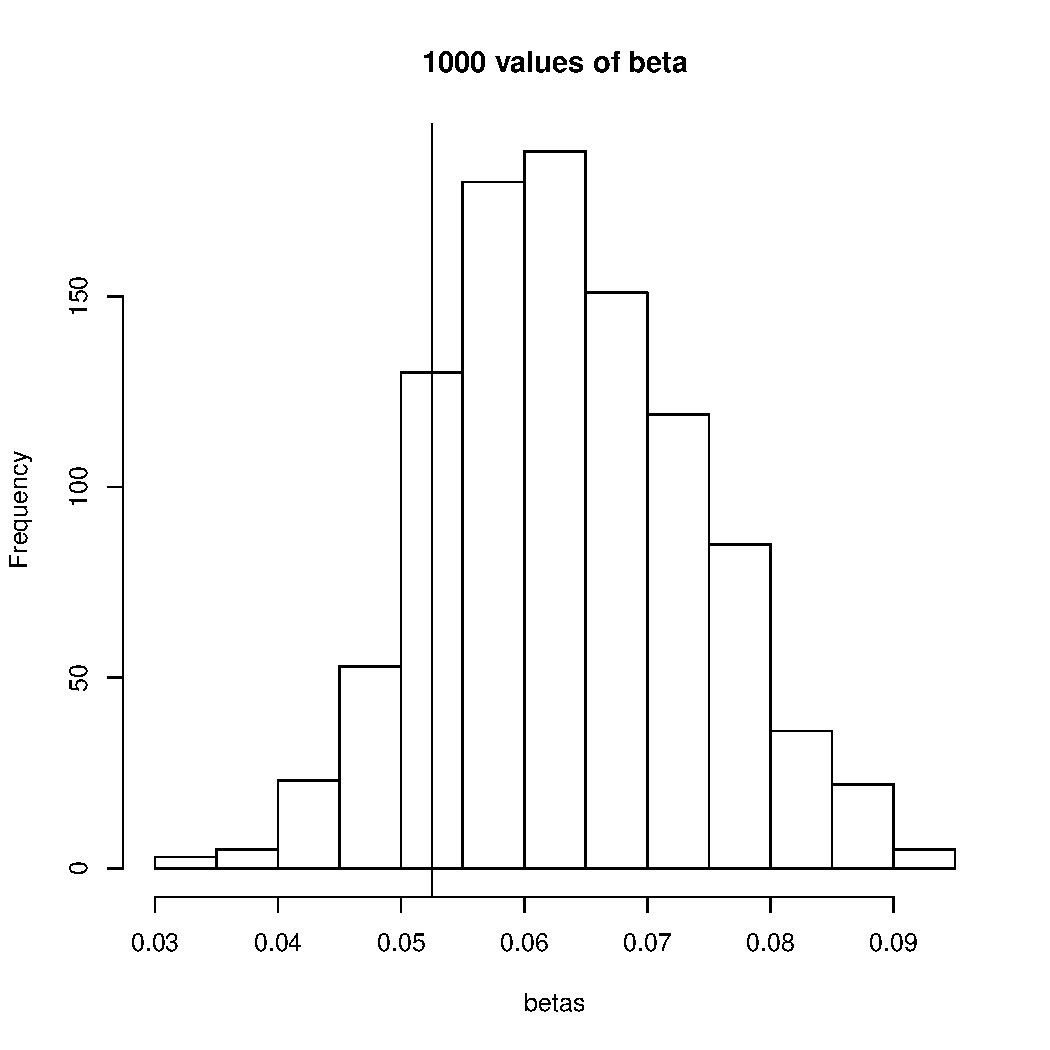
\includegraphics[width=\maxwidth]{figure/unnamed-chunk-11-1} 

\end{knitrout}
The estimate looks biased here. We can have an estimate of the bias with:
\begin{knitrout}
\definecolor{shadecolor}{rgb}{0.969, 0.969, 0.969}\color{fgcolor}\begin{kframe}
\begin{alltt}
\hlkwd{mean}\hlstd{(betas)} \hlopt{-} \hlstd{beta_true}
\end{alltt}
\begin{verbatim}
## [1] 0.011039
\end{verbatim}
\end{kframe}
\end{knitrout}



\end{document}
